\section*{Representação binária}

\begin{frame}[fragile]{Representação em base decimal}

    \metroset{block=fill}
    \begin{block}{Definição}
        A representação de número $n$, em base decimal, consiste na concatenação de $k + 1$ coeficientes $c_i$ tais que
        $$
        n = c_0 + c_1\cdot 10 + c_2\cdot 10^2 + \ldots + c_k\cdot 10^k
        $$
    \end{block}

    \vspace{0.2in}

    Por exemplo,
$$
            2507 = 7 + 0\cdot 10 + 5\cdot 10^2 + 2\cdot 10^3
$$

\end{frame}

\begin{frame}[fragile]{Representação em uma base arbitrária}

    \begin{itemize}
        \item De forma geral, a representação de $n$ em base $b > 1$ é a concatenação de $k + 1$ coeficientes $a_j$ tais que
$$
n = a_0 + a_1\cdot b + a_2\cdot b^2 + \ldots + a_k\cdot b^k
$$

        \item A representação de qualquer inteiro $n$ em base $b$ é única

        \item Esta representação $R(n)$ de $n$ em base $b$ pode ser obtida usando-se recursão e o algoritmo de Euclides: 
$$R(n) = R(q)b + r,$$
        onde $n = bq + r, 0 \leq r < b$
    \end{itemize}

\end{frame}

\begin{frame}[fragile]{Implementação da representação em base arbitrária em C++}
    \inputsnippet{cpp}{5}{19}{codes/representation.cpp}
\end{frame}

\begin{frame}[fragile]{Conversão entre bases}

    \begin{itemize}
        \item A conversão de uma representação em base $a$ para uma base $b$ é, em geral, feita em duas etapas:

        \begin{enumerate}
            \item conversão da base $a$ para uma base pré-determinada (base 10 ou 2, por exemplo);
            \item conversão desta base pré-determinada para a base $b$.
        \end{enumerate}

        \item A primeira etapa é realizada por meio da expansão da representação do número em base $a$

        \item Esta expansão pode ser realizada em $O(k)$ por meio do algoritmo de Horner

        \item A segunda é feita por meio da rotina que obtém a representação
    \end{itemize}

\end{frame}

\begin{frame}[fragile]{Conversão para base decimal}
    \inputsnippet{cpp}{5}{18}{codes/to_decimal.cpp}
\end{frame}

\begin{frame}[fragile]{Representação em base binária}

    \begin{itemize}
        \item A base $b = 2$ é a menor e mais simples dentre todas as bases positivas

        \item Os únicos dois dígitos possíveis em $R(n)$ são \code{cpp}{0} e \code{cpp}{1}

        \item Internamente, os computadores armazenam números inteiros em sua representação binária

        \item É possível comparar diretamente dois números em base binária, sem a necessidade de convertê-los para a base decimal

        \item Para isso, uma vez alinhados o número de dígitos (com zeros à esquerda, se necessário), vale a comparação lexicográfica

        \item Do mesmo modo, é possível somar diretamente dois números em base binária

        \item Uma vez alinhados, a soma de dígitos distintos resulta em \code{cpp}{1}; a soma de dois zeros é \code{cpp}{0}; a soma de dois uns resulta em \code{cpp}{0} e um novo \code{cpp}{1} é adicionado à próxima posição (vai um, \textit{carry})
    \end{itemize}

\end{frame}

\begin{frame}[fragile]{Visualização da soma em base binária}

    \begin{figure}
        \centering
        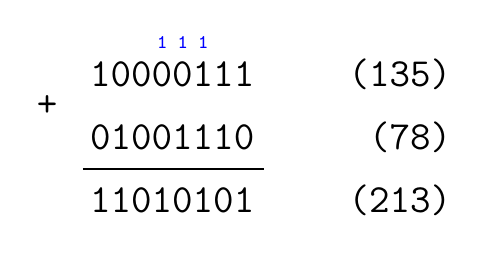
\begin{tikzpicture}
            \node[anchor=east] at (5.55, 3.4) { \scriptsize \textcolor{blue}{\texttt{1  1  1  }} };
            \node[anchor=east] at (6, 3) { \Large \texttt{10000111} };
            \node[anchor=east] at (8.5, 3) { \Large \texttt{(135)} };
            \node[anchor=east] at (6, 2.2) { \Large \texttt{01001110} };
            \node[anchor=east] at (8.5, 2.2) { \Large \texttt{(78)} };
            \node[anchor=east] at (3.5, 2.6) { \Large \texttt{+} };

            \draw[thick] (3.7, 1.8) -- (6, 1.8);

            \node[anchor=east] at (6, 1.4) { \Large \texttt{11010101} };
            \node[anchor=east] at (8.5, 1.4) { \Large \texttt{(213)} };
        \end{tikzpicture}
    \end{figure}

\end{frame}

\begin{frame}[fragile]{\it Overflow}

    \begin{itemize}
        \item Nas linguagens de programação, o número de \textit{bits} usados na representação de inteiros é limitado

        \item Por exemplo, em C/C++, variáveis do tipo \code{cpp}{int}  ocupam, em geral, 32 \textit{bits} (o mesmo espaço em memória que uma palavra do processador)

        \item Variáveis \code{cpp}{long long}, em geral, ocupam 64 \textit{bits}

        \item Esta limitação de espaço pode levar ao \textit{overflow}: quando o limite é atingido, os \textit{bits} que excedem o tamanho máximo ``transbordam'', ficando apenas aqueles que se encontram dentro do limite de espaço

        \item O \textit{overflow} pode levar a resultados inesperados e deve ser tratado com cuidado e atenção
    \end{itemize}

\end{frame}

\begin{frame}[fragile]{Visualização do {\it overflow} em variáveis de 8 {\it bits}}

    \begin{figure}
        \centering

        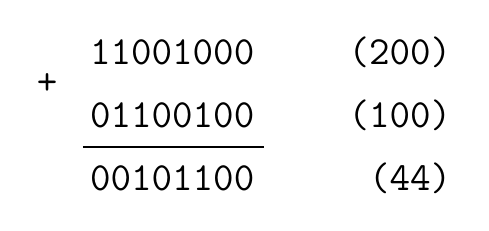
\begin{tikzpicture}
            \node[anchor=east] at (6, 3) { \Large \texttt{11001000} };
            \node[anchor=east] at (8.5, 3) { \Large \texttt{(200)} };
            \node[anchor=east] at (6, 2.2) { \Large \texttt{01100100} };
            \node[anchor=east] at (8.5, 2.2) { \Large \texttt{(100)} };
            \node[anchor=east] at (3.5, 2.6) { \Large \texttt{+} };

            \draw[thick] (3.7, 1.8) -- (6, 1.8);

            \node[anchor=east] at (6, 1.4) { \Large \texttt{00101100} };
            \node[anchor=east] at (8.5, 1.4) { \Large \texttt{(44)} };
        \end{tikzpicture}

    \end{figure}

\end{frame}

\begin{frame}[fragile]{Representação binária de números negativos}

    \begin{itemize}
        \item Para representar número negativos, utiliza-se o fato de que $n + (-n) = 0$

        \item Assim, a representação de $-n$ seria um número tal que, somado com $n$, daria resto zero

        \item Devido ao \textit{overflow}, tal número existe e é denominado complemento de dois de $n$

        \item Por exemplo, em variáveis de 8 \textit{bits} de tamanho, o complemento de dois de $77$ é $179$, pois $77 + 179 = 256 = 0$

        \item O complemento de dois pode ser obtido diretamente, sem necessidade de uma subtração

        \item Basta inverter os \textit{bits} da representação binária de $n$ e somar um ao resultado

        \item Desta maneira, o \textit{bit} mais significativo diferencia os números positivos (zero) dos negativos (um)
    \end{itemize}

\end{frame}

\begin{frame}[fragile]{Visualização do complemento de dois de $77$}

    \begin{figure}
        \centering

        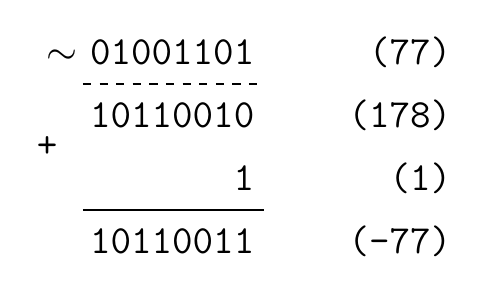
\begin{tikzpicture}
            \node[anchor=east] at (6, 3.8) { \Large $\sim$ \texttt{01001101} };
            \node[anchor=east] at (8.5, 3.8) { \Large \texttt{(77)} };
            \draw[thick,dashed] (3.7, 3.4) -- (6, 3.4);

            \node[anchor=east] at (6, 3) { \Large \texttt{10110010} };
            \node[anchor=east] at (8.5, 3) { \Large \texttt{(178)} };
            \node[anchor=east] at (6, 2.2) { \Large \texttt{1} };
            \node[anchor=east] at (8.5, 2.2) { \Large \texttt{(1)} };
            \node[anchor=east] at (3.5, 2.6) { \Large \texttt{+} };

            \draw[thick] (3.7, 1.8) -- (6, 1.8);

            \node[anchor=east] at (6, 1.4) { \Large \texttt{10110011} };
            \node[anchor=east] at (8.5, 1.4) { \Large \texttt{(-77)} };
        \end{tikzpicture}

    \end{figure}

\end{frame}
